\section{ComponentAbstract Klassenreferenz}
\label{classComponentAbstract}\index{ComponentAbstract@{ComponentAbstract}}
Klassendiagramm für ComponentAbstract::\begin{figure}[H]
\begin{center}
\leavevmode
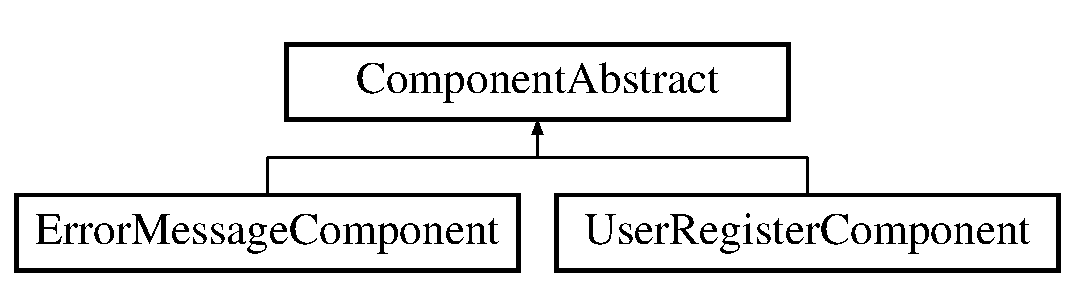
\includegraphics[height=2cm]{classComponentAbstract}
\end{center}
\end{figure}
\subsection*{Öffentliche Methoden}
\begin{CompactItemize}
\item 
{\bf ComponentAbstract} (\$instanceID, \$instanceName, \&\$smartyObj)
\item 
{\bf setClassName} (\$className)
\item 
{\bf getComponentName} ()
\item 
{\bf getComponentInstanceName} ()
\item 
{\bf getComponentID} ()
\end{CompactItemize}
\subsection*{Öffentliche Attribute}
\begin{CompactItemize}
\item 
{\bf \$\_\-name}
\item 
{\bf \$\_\-instanceName}
\item 
{\bf \$\_\-instanceId}
\item 
{\bf \$\_\-componentVarsArr}
\item 
{\bf \$\_\-template}
\item 
{\bf \$\_\-valuesArr}
\item 
{\bf \$\_\-formValuesArr} = null
\item 
{\bf \$\_\-errorValuesArr} = null
\item 
{\bf \$\_\-smartyRef} = null
\end{CompactItemize}


\subsection{Ausführliche Beschreibung}


Definiert in Zeile 7 der Datei ComponentAbstract.php.

\subsection{Dokumentation der Elementfunktionen}
\index{ComponentAbstract@{ComponentAbstract}!ComponentAbstract@{ComponentAbstract}}
\index{ComponentAbstract@{ComponentAbstract}!ComponentAbstract@{ComponentAbstract}}
\subsubsection{\setlength{\rightskip}{0pt plus 5cm}ComponentAbstract.ComponentAbstract (\$ {\em instanceID}, \$ {\em instanceName}, \&\$ {\em smartyObj})}\label{classComponentAbstract_ad4bd12fec470997357118135d8ea17d}


Construnctor

\begin{Desc}
\item[Parameter:]
\begin{description}
\item[{\em string}]\$instanceID \item[{\em string}]\$instanceName \item[{\em Smarty}]\$smartyObj \end{description}
\end{Desc}
\begin{Desc}
\item[Rückgabe:]IComponent \end{Desc}


Definiert in Zeile 80 der Datei ComponentAbstract.php.\index{ComponentAbstract@{ComponentAbstract}!setClassName@{setClassName}}
\index{setClassName@{setClassName}!ComponentAbstract@{ComponentAbstract}}
\subsubsection{\setlength{\rightskip}{0pt plus 5cm}ComponentAbstract.setClassName (\$ {\em className})}\label{classComponentAbstract_b22de345ea6ddc4473566830a4f3d11f}


Set class name - workaround for php4

\begin{Desc}
\item[Parameter:]
\begin{description}
\item[{\em string}]\$className \end{description}
\end{Desc}


Definiert in Zeile 92 der Datei ComponentAbstract.php.\index{ComponentAbstract@{ComponentAbstract}!getComponentName@{getComponentName}}
\index{getComponentName@{getComponentName}!ComponentAbstract@{ComponentAbstract}}
\subsubsection{\setlength{\rightskip}{0pt plus 5cm}ComponentAbstract.getComponentName ()}\label{classComponentAbstract_54022cd983b1da389d452dc5e5f958ba}


Get component name

\begin{Desc}
\item[Rückgabe:]string \end{Desc}


Definiert in Zeile 102 der Datei ComponentAbstract.php.\index{ComponentAbstract@{ComponentAbstract}!getComponentInstanceName@{getComponentInstanceName}}
\index{getComponentInstanceName@{getComponentInstanceName}!ComponentAbstract@{ComponentAbstract}}
\subsubsection{\setlength{\rightskip}{0pt plus 5cm}ComponentAbstract.getComponentInstanceName ()}\label{classComponentAbstract_f398fba12f1cc63c039e5f656251da57}


Gets Instance name

\begin{Desc}
\item[Rückgabe:]string \end{Desc}


Definiert in Zeile 111 der Datei ComponentAbstract.php.\index{ComponentAbstract@{ComponentAbstract}!getComponentID@{getComponentID}}
\index{getComponentID@{getComponentID}!ComponentAbstract@{ComponentAbstract}}
\subsubsection{\setlength{\rightskip}{0pt plus 5cm}ComponentAbstract.getComponentID ()}\label{classComponentAbstract_e4e9d61703d858e0c5290d52fb57edd8}


gets componentID

\begin{Desc}
\item[Rückgabe:]string \end{Desc}


Definiert in Zeile 120 der Datei ComponentAbstract.php.

Wird benutzt von UserRegisterComponent.redender().

\subsection{Dokumentation der Datenelemente}
\index{ComponentAbstract@{ComponentAbstract}!\$\_\-name@{\$\_\-name}}
\index{\$\_\-name@{\$\_\-name}!ComponentAbstract@{ComponentAbstract}}
\subsubsection{\setlength{\rightskip}{0pt plus 5cm}ComponentAbstract.\$\_\-name}\label{classComponentAbstract_5fefdf56492529f0ead1db60f52f9be5}




Definiert in Zeile 13 der Datei ComponentAbstract.php.\index{ComponentAbstract@{ComponentAbstract}!\$\_\-instanceName@{\$\_\-instanceName}}
\index{\$\_\-instanceName@{\$\_\-instanceName}!ComponentAbstract@{ComponentAbstract}}
\subsubsection{\setlength{\rightskip}{0pt plus 5cm}ComponentAbstract.\$\_\-instanceName}\label{classComponentAbstract_96f1c8ded538716ee1bb01cebd8096c2}




Definiert in Zeile 19 der Datei ComponentAbstract.php.\index{ComponentAbstract@{ComponentAbstract}!\$\_\-instanceId@{\$\_\-instanceId}}
\index{\$\_\-instanceId@{\$\_\-instanceId}!ComponentAbstract@{ComponentAbstract}}
\subsubsection{\setlength{\rightskip}{0pt plus 5cm}ComponentAbstract.\$\_\-instanceId}\label{classComponentAbstract_330cf42ad02fe6ef9abda121098c5be7}




Definiert in Zeile 26 der Datei ComponentAbstract.php.\index{ComponentAbstract@{ComponentAbstract}!\$\_\-componentVarsArr@{\$\_\-componentVarsArr}}
\index{\$\_\-componentVarsArr@{\$\_\-componentVarsArr}!ComponentAbstract@{ComponentAbstract}}
\subsubsection{\setlength{\rightskip}{0pt plus 5cm}ComponentAbstract.\$\_\-componentVarsArr}\label{classComponentAbstract_85cf4e9e9d662d707f937fe1c41294cb}




Definiert in Zeile 33 der Datei ComponentAbstract.php.\index{ComponentAbstract@{ComponentAbstract}!\$\_\-template@{\$\_\-template}}
\index{\$\_\-template@{\$\_\-template}!ComponentAbstract@{ComponentAbstract}}
\subsubsection{\setlength{\rightskip}{0pt plus 5cm}ComponentAbstract.\$\_\-template}\label{classComponentAbstract_d2192ff8ab4b3524b92ab9fe4cce9525}




Definiert in Zeile 40 der Datei ComponentAbstract.php.\index{ComponentAbstract@{ComponentAbstract}!\$\_\-valuesArr@{\$\_\-valuesArr}}
\index{\$\_\-valuesArr@{\$\_\-valuesArr}!ComponentAbstract@{ComponentAbstract}}
\subsubsection{\setlength{\rightskip}{0pt plus 5cm}ComponentAbstract.\$\_\-valuesArr}\label{classComponentAbstract_fe9d5e8084355b0b03540cffb33c2668}




Definiert in Zeile 47 der Datei ComponentAbstract.php.\index{ComponentAbstract@{ComponentAbstract}!\$\_\-formValuesArr@{\$\_\-formValuesArr}}
\index{\$\_\-formValuesArr@{\$\_\-formValuesArr}!ComponentAbstract@{ComponentAbstract}}
\subsubsection{\setlength{\rightskip}{0pt plus 5cm}ComponentAbstract.\$\_\-formValuesArr = null}\label{classComponentAbstract_7594e382de0b5a9184fe8aa5de307fc0}




Definiert in Zeile 55 der Datei ComponentAbstract.php.\index{ComponentAbstract@{ComponentAbstract}!\$\_\-errorValuesArr@{\$\_\-errorValuesArr}}
\index{\$\_\-errorValuesArr@{\$\_\-errorValuesArr}!ComponentAbstract@{ComponentAbstract}}
\subsubsection{\setlength{\rightskip}{0pt plus 5cm}ComponentAbstract.\$\_\-errorValuesArr = null}\label{classComponentAbstract_dde2cc0b819bf64b336eb2f6f4e0b79c}




Definiert in Zeile 62 der Datei ComponentAbstract.php.\index{ComponentAbstract@{ComponentAbstract}!\$\_\-smartyRef@{\$\_\-smartyRef}}
\index{\$\_\-smartyRef@{\$\_\-smartyRef}!ComponentAbstract@{ComponentAbstract}}
\subsubsection{\setlength{\rightskip}{0pt plus 5cm}ComponentAbstract.\$\_\-smartyRef = null}\label{classComponentAbstract_98c8fb6309c207d60d3398df2b8470d9}




Definiert in Zeile 70 der Datei ComponentAbstract.php.

Die Dokumentation für diese Klasse wurde erzeugt aufgrund der Datei:\begin{CompactItemize}
\item 
{\bf ComponentAbstract.php}\end{CompactItemize}
